\documentclass[12pt, a4paper, oneside]{book}
\usepackage[hidelinks]{hyperref}
\usepackage[slovak]{babel}
\usepackage{epsfig}
\usepackage{epstopdf}
\usepackage[chapter]{algorithm}
\usepackage{algorithmic}
\usepackage{listings}
\usepackage{amsmath}
\usepackage{amssymb}
\usepackage{graphicx}
\usepackage{multirow}
\usepackage{color}
\usepackage{url}
\usepackage[utf8]{inputenc}
\usepackage[T1]{fontenc}
\usepackage{setspace}
\usepackage{tabularx}
\usepackage{textcomp}
\usepackage{caption}
\usepackage{natbib}

\setstretch{1.5}
%\renewcommand\baselinestretch{1.5} % riadkovanie jeden a pol

% pekne pokope definujeme potrebne udaje
\newcommand\mftitle{Klaboratívny grafický editor pre MediaWiki}
\newcommand\mfthesistype{Diplomová práca}
\newcommand\mfauthor{Bc. Martin Krasňan}
\newcommand\mfadvisor{doc. RNDr. Zuzana Kubincová, PhD.}
\newcommand\mfplacedate{Bratislava, 2018}
\newcommand\mfuniversity{UNIVERZITA KOMENSKÉHO V BRATISLAVE}
\newcommand\mffaculty{FAKULTA MATEMATIKY, FYZIKY A INFORMATIKY}
\newcommand{\sub}[1]{$_{\text{#1}}$}
\newcommand{\reference}[1]{č.~\ref{#1}}
\newcommand{\imageHeight}{150px}

\ifx\pdfoutput\undefined\relax\else\pdfinfo{ /Title (\mftitle) /Author (\mfauthor) /Creator (PDFLaTeX) } \fi

\begin{document}

\frontmatter

\thispagestyle{empty}

\noindent
\begin{minipage}{\textwidth}
\begin{center}
\textbf{\mfuniversity \\
\mffaculty}
\end{center}
\end{minipage}

\vfill
\begin{figure}[!hbt]
	\begin{center}
		
\includegraphics{images/logo_fmph}
		\label{img:logo}
	\end{center}
\end{figure}
\begin{center}
	\begin{minipage}{0.8\textwidth}
		\centerline{\textbf{\Large\MakeUppercase{\mftitle}}}
		\smallskip
		\centerline{\mfthesistype}
	\end{minipage}
\end{center}
\vfill
2018 \hfill
\mfauthor
\eject 
% koniec obalu

\thispagestyle{empty}

\noindent
\begin{minipage}{\textwidth}
\begin{center}
\textbf{\mfuniversity \\
\mffaculty}
\end{center}
\end{minipage}

\vfill
\begin{figure}[!hbt]
\begin{center}

\includegraphics{images/logo_fmph_dark}
\label{img:logo_dark}
\end{center}
\end{figure}
\begin{center}
\begin{minipage}{0.8\textwidth}
\centerline{\textbf{\Large\MakeUppercase{\mftitle}}}
\smallskip
\centerline{\mfthesistype}
\end{minipage}
\end{center}
\vfill
\begin{tabular}{l l}
%Registration number: & 40a99bd8-3cb6-4534-9330-c7fd9b5e5ca4 \\
Študijný program: & Aplikovaná informatika\\
Študijný odbor: & 2511 Aplikovaná informatika\\
Školiace pracovisko: & Katedra aplikovanej informatiky\\
Školiteľ: & \mfadvisor
\end{tabular}
\vfill
\noindent
\mfplacedate \hfill
\mfauthor
\eject 
% koniec titulneho listu

%\thispagestyle{empty}
%\includegraphics[width=\textwidth]{images/zadanie}
%\vfill
%\eject
% koniec zadania

\thispagestyle{empty}


\begin{figure}[H]
\begin{center}
\makebox[\textwidth]{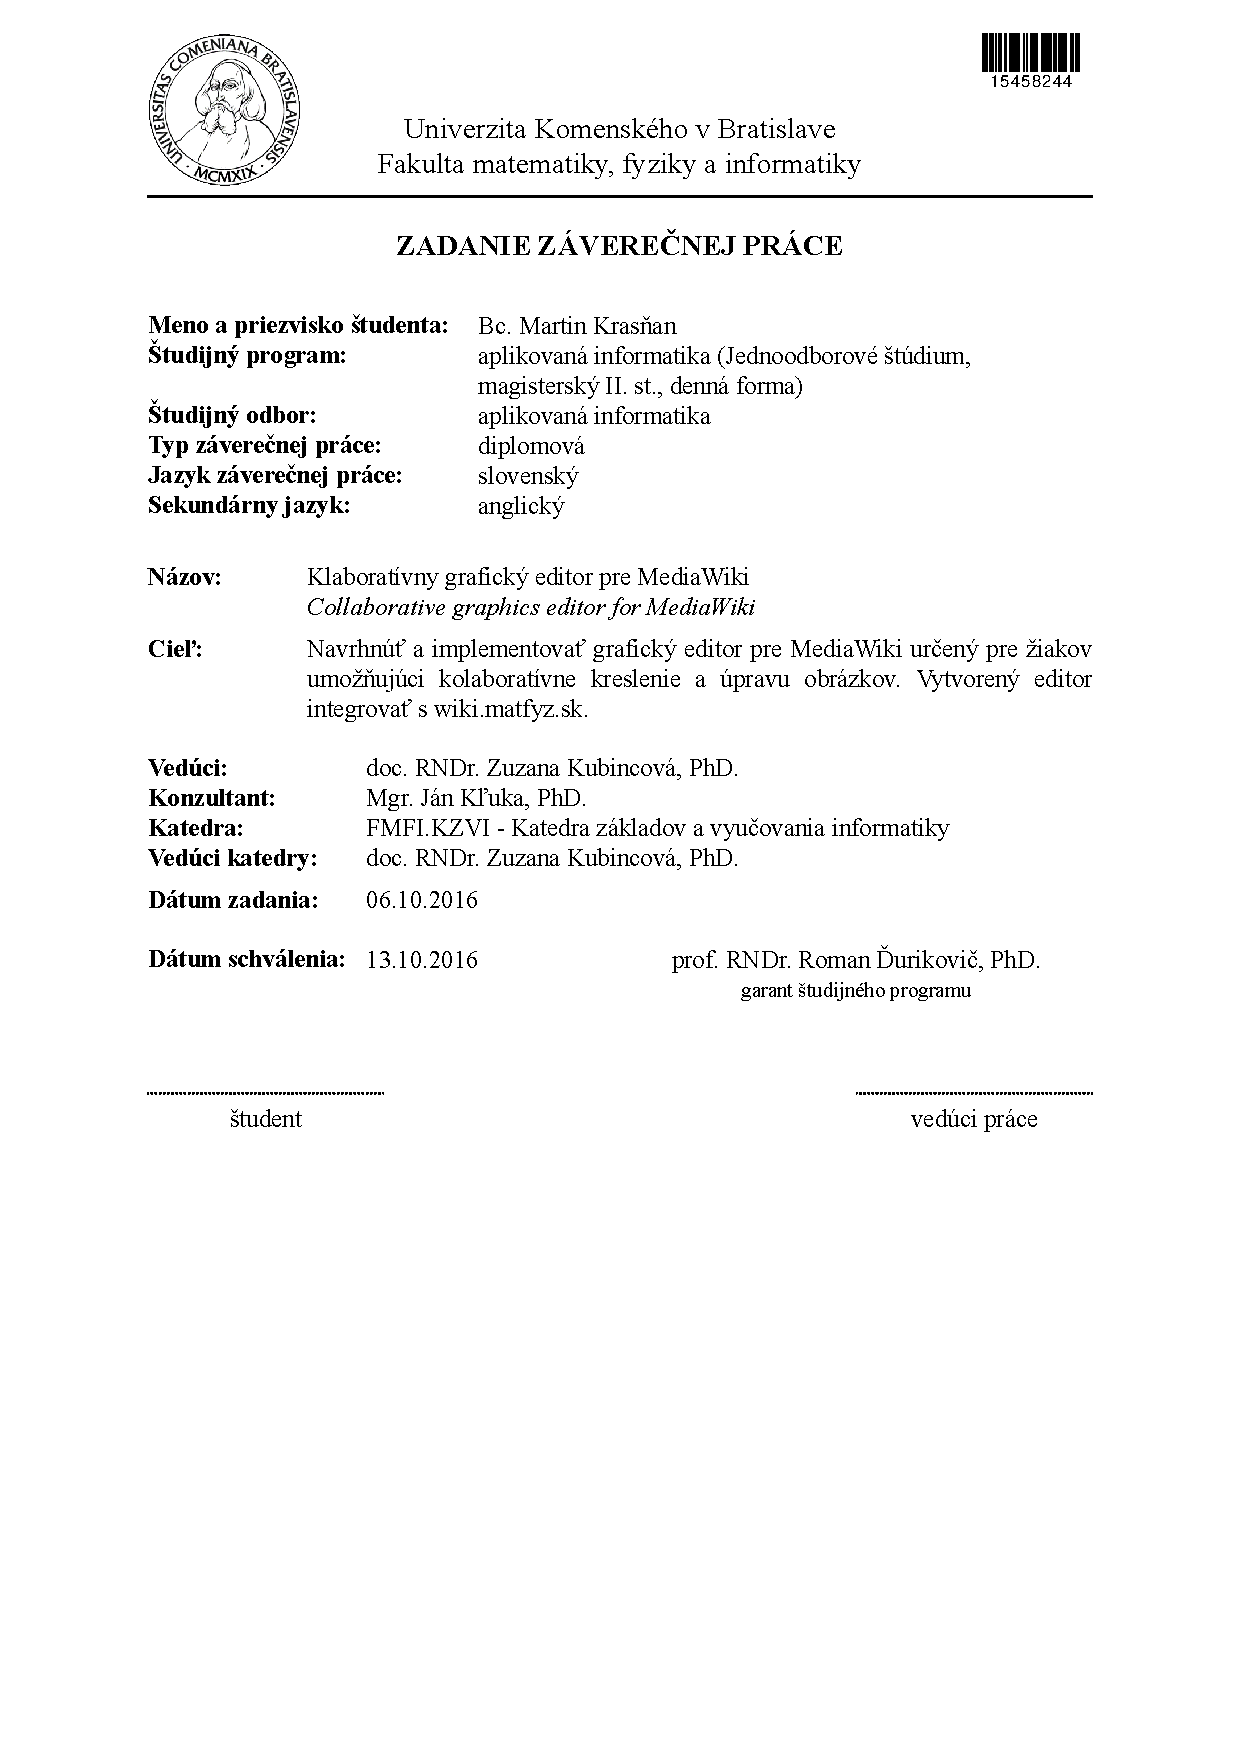
\includegraphics[width=\paperwidth]{images/zadaniedp}}
\label{img:zadanie}
\end{center}
\end{figure}

{~}\vspace{12cm}

\noindent
\begin{minipage}{0.25\textwidth}~\end{minipage}
\begin{minipage}{0.75\textwidth}
Čestne vyhlasujem, že som túto diplomovú prácu vypracoval samostatne pod vedením doc. RNDr. Zuzany Kubincovej, PhD., s použitím zdrojov uvedených v zozname použitej literatúry.
\newline \newline
\end{minipage}
\vfill
~ \hfill {\hbox to 6cm{\dotfill}} \\
\mfplacedate \hfill \mfauthor
\vfill\eject 
% koniec prehlasenia

\chapter*{Poďakovanie}\label{chap:thank_you}
...podakovanie...
\vfill\eject 
% koniec podakovania

\chapter*{Abstrakt}\label{chap:abstract_sk}
...abstrakt sk...
~\\
Kľúčové slová: klucove, slova, sk, ...
\vfill\eject 

\chapter*{Abstract}\label{chap:abstract_en}
...abstract en...

~\\
Keywords: keywords, en, ...
\vfill\eject 
% koniec abstraktov

\tableofcontents

\mainmatter

% treba este prejst dokument ci je kod spravne formatovany
\input 01intro.tex
\input 02motivation.tex
\input 03issues_overview.tex
\input 04previous_solutions.tex
\input 05proposal.tex
\input 06implementation.tex
\input 07results.tex
\input 08conclusion.tex

\backmatter

\nocite{*}
\bibliographystyle{alpha}
\bibliography{references}

\listoffigures

\end{document}